%%% PREGUNTA

\begin{ejercicio}\label{ej:12}
	Sea $\Omega X$ el espacio de lazos de un espacio basado $(X,x_0)$, equipada con la topolog\'ia
	compacto-abierta. Entonces las funciones
	\[
		\mu:\Omega X \times \Omega X \lra \Omega X \quad\text{y}\quad \la:\Omega X \lra \Omega X
	\]
	definidas por $\mu(\alpha,\beta)=\alpha*\beta$ y $\la(\alpha)=\bar{\alpha}$ son funciones
	continuas. En particular $\Omega X$ es un $H$-grupo.
\end{ejercicio}

%%% RESPUESTA
\begin{proof}% 

Recuerda que la topolog\'ia compacto-abierta tiene como subase a todos los conjuntos de la forma
\[
	B(K,U):=\{\alpha\in\Omega X \mid \alpha[K]\subseteq U\}
\]
donde $K\subseteq I$ es compacto y $U\subseteq X$ es abierto. A $K$ la puedo separar como la uni\'on
de los dos compactos $K_1:=K\cap[0,\tfrac{1}{2}]$ y $K_2=K\cap[\tfrac{1}{2},1]$ ($K_i$ es compacto por
ser subespacio cerrado de un compacto). Entonces $K=K_1\cup K_2$ y $B(K,U)=B(K_1,U)\cap B(K_2,U)$ porque
$\alpha[K_1],\alpha[K_2]\subseteq U$ si y s\'olo si $\alpha[K_1]\cup\alpha[K_2]=\alpha[K]\subseteq U$.

Por lo tanto para probar continuidad
basta verificar que $\mu^{-1}[B(K,U)]$ y $\la^{-1}[B(K,U)]$ son abiertos en $\Omega X\times\Omega X$
y $\Omega X$ respectivamente, para todo compacto $K\subseteq I$ y abierto $U\subseteq X$.

Sea $K\subseteq I$ compacto y $U\subseteq X$ abierto. Afirmo que:
\[
	\mu^{-1}[B(K,U)]=B(2K_1,U)\times B(2K_2-1,U) \quad\text{y}\quad \la^{-1}[B(K,U)]=B(1-K,U)
\]
donde $2K_1$ es la imagen de $K_1$ bajo la funci\'on continua $x\mapsto 2x$; observa que $2K_1$ es
compacto. De manera similar defino $2K_2-1$ y $1-K$.

Para la primera igualdad observa que:
\begin{align*}
	(\alpha,\beta)\in\mu^{-1}[B(K,U)] & \quad\iff\quad
        \mu(\alpha,\beta)[K]=(\alpha*\beta)[K]=(\alpha*\beta)[K_1]\cup(\alpha*\beta)[K_2]\subseteq U\\&
        \quad\iff\quad (\alpha*\beta)[K_1]\subseteq U\;\;\text{y}\;\;(\alpha*\beta)[K_2]\subseteq U.
\end{align*}
Ahora si $s\in K_1$ entonces $(\alpha*\beta)(s)=\alpha(2s)$ y as\'i $\alpha[2K_1]=(\alpha*\beta)[K_1]$.
Por lo tanto
\[
	(\alpha*\beta)[K_1]=
	\alpha[2K_1]\subseteq U \quad\iff\quad
	\alpha\in B(2K_1,U), 
\]
y similarmente:
\[
	(\alpha*\beta)[K_2]=
	\beta[2K_2-1]\subseteq U \quad\iff\quad
	\beta\in B(2K_2-1,U), 
\]

Con esto concluyo que:
\[
	(\alpha,\beta)\in\mu^{-1}[B(K,U)] \quad\iff\quad (\alpha,\beta)\in B(2K_1,U)\times B(2K_2-1,U)
\]
y as\'i $\mu^{-1}[B(K,U)]=B(2K_1,U)\times B(2K_2-1,U)$ es abierto (por ser producto de sub\'asicos).

Por \'ultimo, como $\la(\alpha)(s)=\bar{\alpha}(s)=\alpha(1-s)$, tengo que $\alpha[1-K]=\bar{\alpha}[K]$
An\'alogamente concluyo que $\alpha\in\la^{-1}[B(K,U)]$ si y s\'olo si $\alpha\in B(1-K,U)$ y as\'i
$\la^{-1}[B(K,U)]=B(1-K,U)$ es abierto.

Con esto termino la prueba. La figura%
\begin{figure}
  \centering
  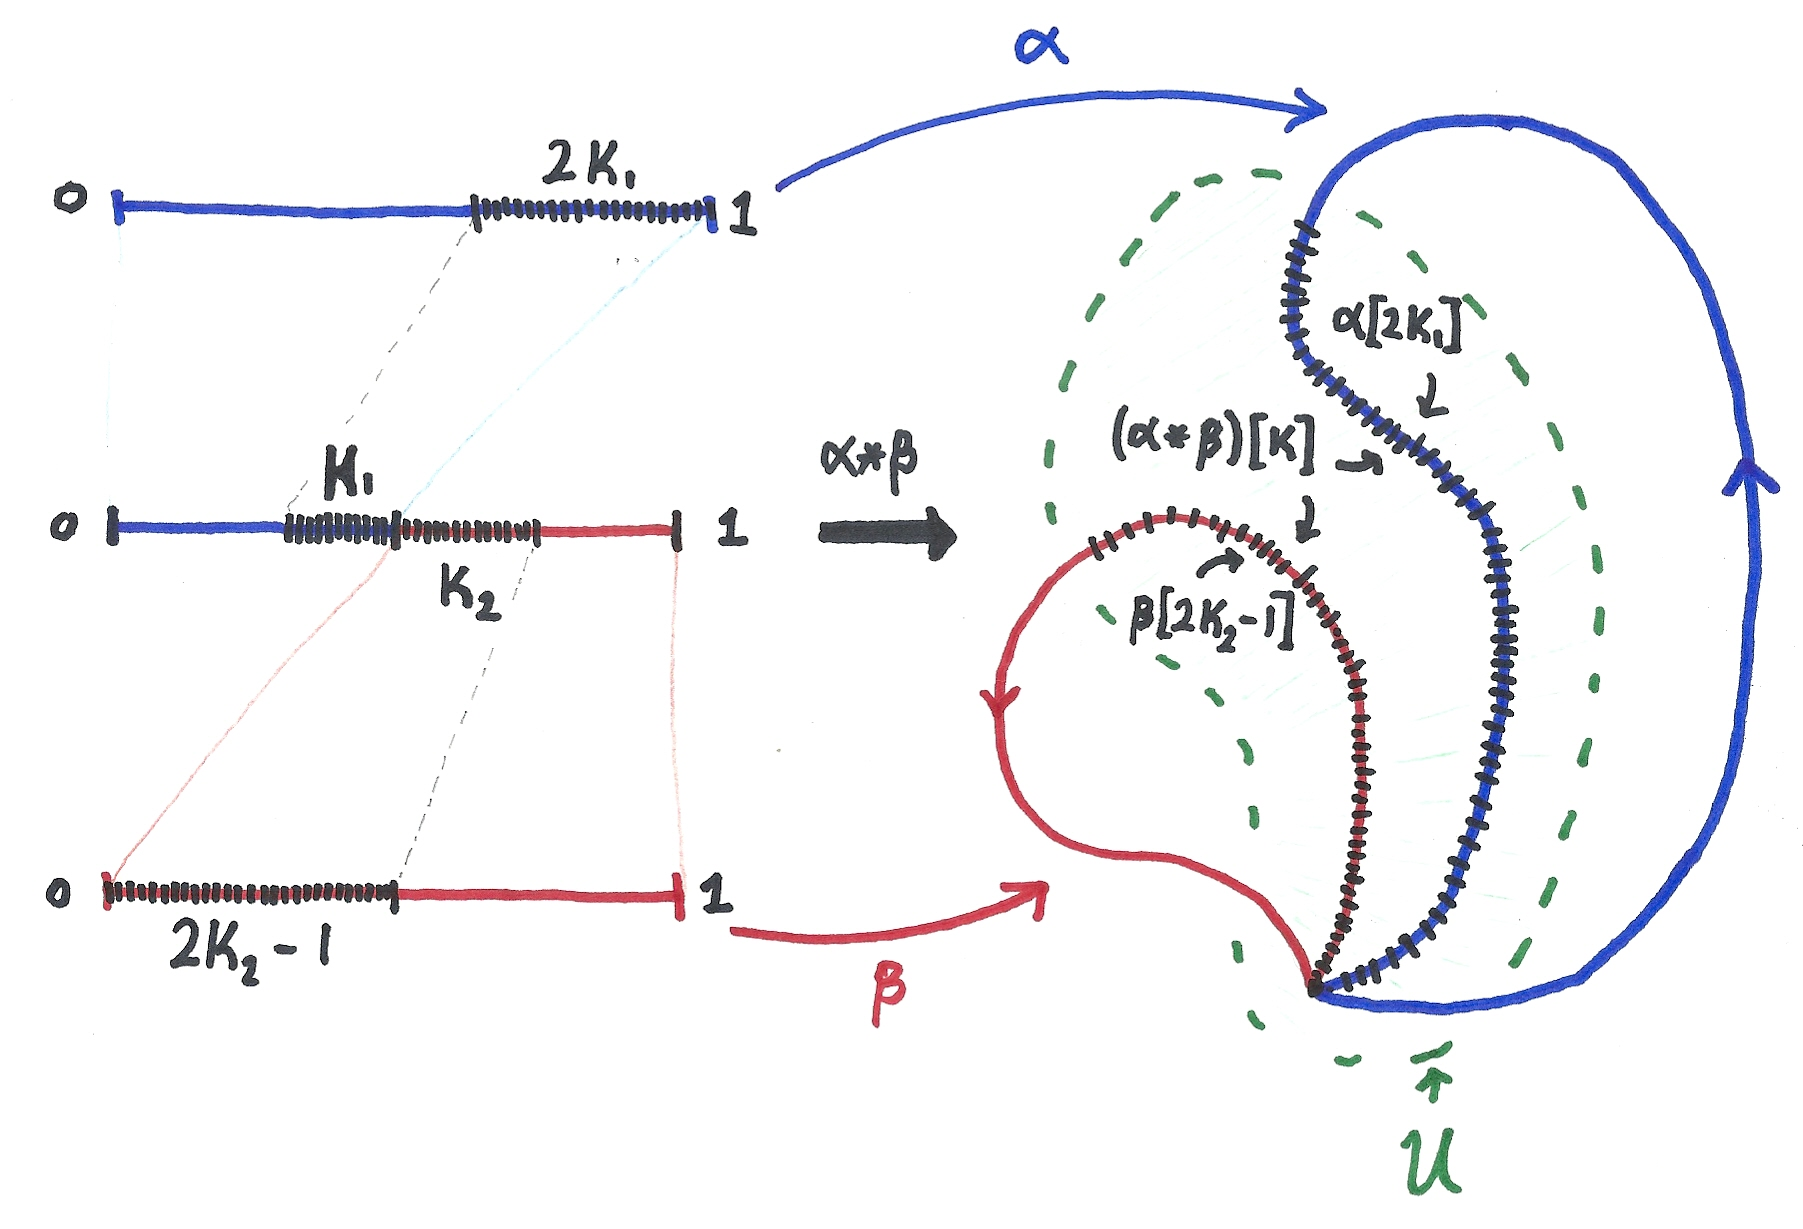
\includegraphics[scale=0.17]{omega_hgrupo}
  \caption{La multiplicaci\'on en $\Omega X$ es continua.}
  \label{fig:omega_hgrupo}
\end{figure}
\ref{fig:omega_hgrupo} ilustra esta demostraci\'on.


\end{proof}%

